\documentclass[12pt]{article}
\usepackage{amsmath}
\usepackage{amssymb}
\usepackage{graphicx}
\usepackage{listings}
\usepackage{xcolor}
\usepackage{xparse}
\usepackage{comment}
\usepackage{dirtree}
\usepackage{csquotes}
\usepackage{subfig}
\usepackage{physics}
\usepackage{algorithm}
\usepackage{amsfonts}
\usepackage{algorithmicx}
\usepackage{algpseudocode}
\usepackage{siunitx}
\usepackage{upquote}

\usepackage{tikz}
\usetikzlibrary{positioning}
\usetikzlibrary{intersections}
\usetikzlibrary{backgrounds}
\usetikzlibrary{mindmap}
\usetikzlibrary{shadows}
\usetikzlibrary{trees}
\usetikzlibrary{shapes.misc}
\usetikzlibrary{arrows.meta}
\usetikzlibrary{decorations.pathmorphing}

\usepackage{hyperref}

% \usepackage[margin=0.25in]{geometry}
\usepackage{pgfplots}
\pgfplotsset{width=10cm,compat=1.9}

% We will externalize the figures
% \usepgfplotslibrary{external}
% \tikzexternalize

\hypersetup{
    colorlinks,
    linkcolor={red!50!black},
    citecolor={blue!50!black},
    urlcolor={blue!80!black}
}

% Rename "Contents" to "Summary"
\renewcommand*\contentsname{Summary}

% Register codeword as a command
\NewDocumentCommand{\codeword}{v}{%
\texttt{\textcolor{darkgray}{#1}}%
}

% C++
\def\CC{{C\nolinebreak[4]\hspace{-.05em}\raisebox{.4ex}{\tiny\bf ++ }}}

% SymboMath
\def\Symbo{{$\texttt{SymboMath}$}}

% WolframAlpha
\def\Wolf{{{\color{red}Wolfram\color{orange}Alpha}}}

\title{
\textsc{Implementing Symbolic Mathematics in a Statically-Typed Language}\\[2.2cm]

% Title and Subtitle

{\LARGE \bfseries
SymboMath}\\
{\Large\bfseries
Symbolic Mathematics in \CC}
}

% Author
\author{Toby Davis\\[0.2cm]Hampton School}

% Code style
\definecolor{codegreen}{rgb}{0,0.6,0}
\definecolor{codegray}{rgb}{0.5,0.5,0.5}
\definecolor{codepurple}{rgb}{0.58,0,0.82}
\definecolor{backcolour}{rgb}{0.95,0.95,0.92}

\lstdefinestyle{mystyle}{
    backgroundcolor=\color{backcolour},   
    commentstyle=\color{codegreen},
    keywordstyle=\color{magenta},
    numberstyle=\tiny\color{codegray},
    stringstyle=\color{codepurple},
    basicstyle=\ttfamily\footnotesize,
    breakatwhitespace=false,         
    breaklines=true,                 
    captionpos=b,                    
    keepspaces=true,                 
    numbers=left,                    
    numbersep=5pt,                  
    showspaces=false,                
    showstringspaces=false,
    showtabs=false,                  
    tabsize=2
}

\lstset{style=mystyle}

\begin{document}
\maketitle
\thispagestyle{empty}
\vspace{0.5cm}
\hrule
\vspace{1cm}
\begin{abstract} % 150-250 words
While computers excel at solving numerical calculations, it is incredibly difficult to efficiently compute symbolic equations -- i.e., equations including variables, derivatives and integrals. For numerical calculations and the vast majority of software, symbolic mathematics provides very limited benefits. However, in certain applications, such as visual calculators and scientific programs, the ability to manipulate equations algebraically can be incredibly useful.

This paper investigates how symbolic mathematics can be implemented in \CC, an object-oriented, statically-typed language which operates closer to the hardware than languages like Python and Java.
\end{abstract}

\vfill
\newpage

{
  \hypersetup{linkcolor=black}
  \tableofcontents
}

\pagebreak

\section{What is Symbolic Mathematics?} \label{whatisit}

Symbolic mathematics is ``the use of computers to manipulate mathematical equations and expressions in symbolic form, as opposed to manipulating the numerical quantities represented by those symbols''\cite{symbolicdefinition}.  In practice, this means the computer can deal with an expression like $5x+7$, instead of, for example, $5 \cdot 2 + 7$. It is also possible to compute derivatives and, in some cases, integrals, using a symbolic mathematics engine.
 
\subsection{Why is Symbolic Mathematics Useful?} \label{whyuseful}

The most common use-case for  symbolic mathematics is for solving incredibly large, tedious problems, which would be prone to trivial errors if solved by a human \cite{computeraidformathematics}. By providing a computer with suitable instructions and rules, it is possible to answer questions that had been ignored for millennia due to their scale and complexity. Furthermore, the program can evaluate, manipulate and solve equations step-by-step, helping students, researchers and hobbyists understand their problem better.

For example, a huge number of research projects make use of Wolfram Mathematica\cite{mathematica}

Another common use for a symbolic maths engine is to present data in a more human-readable form. For example, \Wolf{} is capable of taking complex, multi-variable equations as inputs and manipulating them to solve equations, plot interactive graphs and provide general solutions to queries.

\subsection{Comparison to Naive Methods}

As mentioned in \ref{whyuseful}, symbolic mathematics engines can directly differentiate or integrate an expression, providing exact answers as opposed to approximations.

\subsubsection{Derivatives}

The derivative of a function is defined with the following expression:

\begin{equation}
\dv{x} f(x) = \lim_{h \rightarrow 0}{\frac{f(x+h)-f(x)}{h}}
\end{equation}

However, this is very difficult for a computer to deal with, due to the limit.

To approximate the derivative of a function, it is possible to use the definition of the derivative without the limit, replacing $h$ with $\epsilon$, where $\epsilon$ is a very small number.

This produces the following expression, which can, in some cases, be suitable for derivative calculations in simple programs.

\begin{equation}
\dv{x} f(x) = \frac{f(x + \epsilon) - f(x)}{\epsilon}
\end{equation}

However, there are many issues with this approach, though the most significant is the lack of precision. Using a relatively large\footnote{The size of $epsilon$ required for a given precision will depend heavily on the function being differentiated.} value of $\epsilon$ will result in a more precise \textit{calculation}, but a less precise \textit{result}. This discrepancy is due to the large difference in the values substituted into $f(x)$.
	
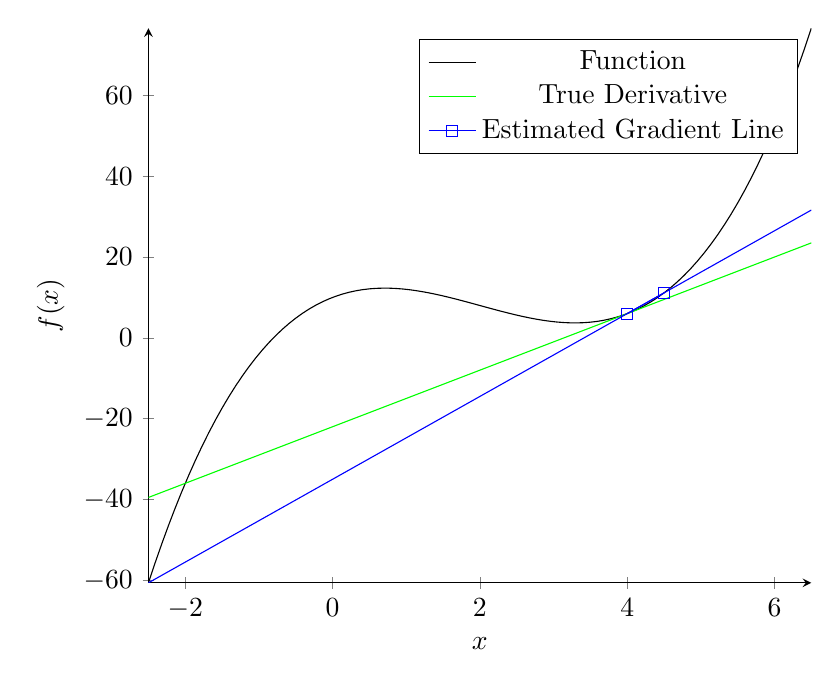
\begin{tikzpicture}
\begin{axis}[
    axis lines = left,
    xlabel = \(x\),
    ylabel = {\(f(x)\)},
]
% Plot the curve
\addplot [
    domain=-2.5:6.5, 
    samples=100, 
    color=black,
]
{x^3-6*x^2+7*x+10};
\addlegendentry{\(\text{Function}\)}

% Plot true gradient
\addplot [
    domain=-2.5:6.5, 
    samples=100, 
    color=green,
]
{7*(x-4)+6};
\addlegendentry{\(\text{True Derivative}\)}

% Plot bad gradient
\addplot[
    color=blue,
    mark=square,
    ]
    coordinates {
    (4, 6)(4.5, 11.125)
    };
    
\addplot [
    domain=-2.5:6.5, 
    samples=100, 
    color=blue,
]
{(41/4)*(x-4)+6};
\addlegendentry{\(\text{Estimated Gradient Line}\)}

\end{axis}
\end{tikzpicture}

The plot above shows $y=x^3-6x^2+7x+10$, along with the true derivative and the estimated derivative, with $\epsilon=0.5$.

The equations below show how the true derivative differs from the approximated one, using two different values of $\epsilon$ to show how greater precision can be achieved.

\begin{equation}
\begin{split}
&\text{Symbolic Derivative} \\
f(x)&=x^3-6x^2+7x+10 \\
g(x)&=\dv{f}{x}=6x^2-12x+7 \\
g(4)&=7
\end{split}
\end{equation}

\begin{equation}
\begin{split}
&\text{Approximated Derivative} \\
f(x)&=x^3-6x^2+7x+10 \\
h(x, \epsilon)&=\dv{f}{x}=\frac{f(x+\epsilon)-f(x)}{\epsilon} \\
h(4, 0.5)&=\frac{41}{4}=10.25 \\
h(4, 1 \cdot 10^{-5})& \approx 7.00005999832
\end{split}
\end{equation}

From the above results, it appears that continually reducing the value of $\epsilon$ will result in more precise results. While this is true numerically, it is not the case for floating-point arithmetic. 

As $\epsilon$ becomes increasingly small, floating point rounding errors will cause the final result to become \textit{less} accurate. It is likely that the resulting gradient will become closer to zero, as, in most cases, the error occurs in the evaluation of $f(x+\epsilon)$:

$$
x+\epsilon \approx x
$$

$$
\therefore f(x+\epsilon) \approx f(x)
$$

$$
\therefore f(x+\epsilon) - f(x) \approx 0
$$

$$
\therefore \frac{\Delta f}{\epsilon} \approx \frac{0}{\epsilon} = 0
$$

For a coarse approximation of a derivative, this method works very well and can be quite efficient\footnote{The efficiency of this will depend on the function itself.}. However, this approach will not allow you to express the exact derivative of a function. For example, you would not be able to compute $\dv{x}x^2=2x$ with a purely numeric algorithm.

\subsubsection{Integration}

Integration is often much more difficult than differentiation, and requires a wide range of different techniques to compute efficiently.

One common method of integrating numerically is with a Riemann sum\cite{riemannsum}. Riemann sums approximate an integral by summing $N$ rectangles with width $w$ and height $f(x)$. In practice, this takes the following form:

$$
\int_{a}^{b}{f(x) \ \text{dx}} = \lim_{N \rightarrow \infty}\left(\sum_{n=0}^{N}{r_1+r_2+r_3+...+r_{n-1}+r_{n}} \right)
$$

\noindent
where $r_m$ is the area of rectangle $m$, and $w=(b-a)N^{-1}$. Substituting these values into the above sum produces the following expression.

$$
\int_{a}^{b}{f(x) \ \text{dx}} = \lim_{N \rightarrow \infty} \left( \sum_{n=0}^{N}{f \left( a+nw \right) w } \right)
$$

The above expression can be written in Python with something as simple as the following function:

\begin{lstlisting}[language=python]
def integrate(f, a, b, N=10):
	tot = 0
	w = (b - a) / N
	for i in range(N):
		tot += f(a + w * i) * w
	return tot
	
#              f(x)=x  a  b   N        result
integrate(lambda x: x, 0, 10, 5    ) # 40.0
integrate(lambda x: x, 0, 10, 10   ) # 45.0
integrate(lambda x: x, 0, 10, 100  ) # 49.5
integrate(lambda x: x, 0, 10, 1000 ) # 49.949999999999996
integrate(lambda x: x, 0, 10, 10000) # 49.99500000000002
\end{lstlisting}

While this implementation works in theory, it is incredibly inefficient and impractical to use for precise calculations. This is because $N$ must be very large, and hence many iterations must be run.

To solve this problem, one could integrate symbolically. This would produce a new, explicit function, into which a value of $x$ can be substituted directly, giving an exact value for the integral.

Unfortunately, symbolically integrating equations is incredibly difficult, especially with a program. However, it is possible, and some methods for achieving it are explained later.

\subsection{Why \CC?}

\CC is a statically-typed language based on C, providing classes, structs, template-meta-programming and more. It is also possible to write highly efficient code in \CC, making it the programming language of choice for many high-performance applications. However, since \CC is statically typed, it adds another layer of complexity to implementing a symbolic mathematics library, as it makes it vastly more complicated to deal with different types for numbers, variables, functions, operations, etc.

If this project were to be implemented in Python, which is dynamically typed, it would be much easier to design a data-structure which could store a symbolic equation and operate on it accordingly because the language does not require the type of a variable to be specified.

\CC also provides a much greater opportunity for code optimisation and more interesting implementations, as well as having far fewer symbolic mathematics libraries available for it \cite{githubmathlibs}. Hence, so a novel implementation could help a wider range of projects. Finally, \CC is easy to integrate into other programming languages, as they are often written in \CC themselves, meaning a \CC library could easily be used in Python, JavaScript, Rust, Julia, etc.

\subsection{What About Automatic Differentiation?}

When researching symbolic mathematics, particularly symbolic \textit{differentiation}, one is bound to come across the term ``automatic differentiation''. This varies from symbolic mathematics in a few significant ways.

Firstly, automatic differentiation does not operate on symbolic equations. Instead, it operates entirely numerically, though may operate on vectors, matrices or arrays -- not just scalar values.

Secondly, automatic differentiation aims to provide a means of \textit{evaluating} the derivative of a function at a given point, not \textit{calculating} it symbolically. This may seem exactly like the approximation methods spoken about earlier, but it does still provide a function for the derivative.

Automatic differentiation is most commonly used in machine-learning applications, where a complex activation function needs to be differentiated in order to make use of the gradient descent algorithm. The reason it's used in such cases is because, given a static, compile-time definition for a function, it is possible to generate another function, also at compile-time, which represents the derivative of the initial function. This means no time needs to be spent at runtime parsing the input and differentiating it before evaluating the result.

\pagebreak
\section{Existing Symbolic Mathematics Libraries}

Pre-existing symbolic mathematics libraries are a good place to start to identify implementation techniques and overall design architectures, as they are shown to work effectively.

$\texttt{mathiu.cpp}$\cite{mathiucpp} is a \CC symbolic mathematics library based heavily on pattern matching. By making use of the $\texttt{match(it)}$ library, $\texttt{mathiu.cpp}$ can combine and compare operations and expressions to form an equation. Differentiation is performed recursively, applying a small set of rules to individual functions and combining them to produce the final result.

Wolfram Mathematica is another program capable of symbolic manipulation of equations. Although Mathematica's code is not available online, there are detailed explanations on the Wolfram Reference website \cite{mathematicainternals} of how it's internal systems handle the data. According to their explanations, Wolfram Mathematica has four fundamental data types:

\begin{align*}
&\texttt{Numbers}
\\
&\texttt{Strings}
\\
&\texttt{Symbols}
\\
&\texttt{General Expressions}
\end{align*}

Everything in the Wolfram Language keeps a reference count, tracking how many other Wolfram Language objects are pointing to it. This allows the language to free anything immediately after the last thing pointing to it is destroyed, saving memory and improving efficiency.

To process the inputs provided to the language, the Wolfram Language first creates an expression representing the input. It then applies all known rules for the contained objects before outputting the result. The important thing to note here is that \textit{all} known rules are applied. This implies that no single rule can achieve the desired result, and that intelligently analysing the expression to identify the most effective rule is not always possible.

Another incredibly powerful symbolic mathematics engine is $\texttt{Symengine}$\cite{symengine}, which implements an incredibly wide range of functions. Analysing the full workings of this library is far beyond the scope of this project. However, at the most basic level, it uses the same reference-counted pointer system used by $\texttt{mathiu.cpp}$, suggesting that this is the optimal design choice for such a program.

\subsection{Issues with the Existing Libraries}

While the existing libraries and frameworks such as Wolfram Mathematics, $\texttt{mathiu.cpp}$ and $\texttt{Symengine}$ are incredibly powerful, they often have one of two major shortcomings -- a lack of features or excessive code size.

Many symbolic mathematics engines implement only a very limited subset of features, and hence are not applicable to large-scale projects. Only a select few projects implement the necessary functions and routines to be used in critical software.

On the other hand, the engines which are capable of handling an extremely wide range of mathematical expressions often contain upwards of 100,000 lines of code, making them difficult and slow to compile, as well as unsuitable for smaller projects.

\pagebreak
\section{\Symbo's Goals} \label{symbogoals}

\Symbo{}, implemented following this paper, is not a fully featured library and does not implement all the possible functions, derivatives, simplification rules, etc. required for an advanced program. It does, however, lay out the groundwork for further implementations to be built on top of.

\Symbo \footnote{\Symbo{} GitHub repository: \href{https://github.com/Pencilcaseman/SymboMathPaper}{https://github.com/Pencilcaseman/SymboMathPaper}.} should be a library usable in any \codeword{CMake} project, and should be wrapped in an easy-to-use, \CC-styled class for easy reuse of variables, equations and functions.

\Symbo{} \textit{could} also support some form of basic equation solving, though this might be outside the scope of simple algebraic manipulation of equations.

\subsection{Numeric Evaluation}

The program should be able to evaluate any numeric expression involving the four basic arithmetic operations, as well as exponentiation, trigonometry and nth-roots.

\subsection{Functions}

It should be easy to register custom functions with procedures to evaluate, differentiate and potentially integrate them. There should also be a wide set of common functions implemented by default, including trigonometry, logarithms and exponents, square roots, etc.

\subsection{Variables}

\Symbo{} must be able to support user-defined variables, including value substitution, manipulation of equations including variables and potentially simplification of expressions containing variables (see \ref{simplificationgoal}). Variables should act like any other object within the data structure of an equation, and operations applied to them should perform as expected, with no unwanted side-effects.

\subsection{Calculus}

The primary data structure used in \Symbo{} should be easily differentiated given that every function being used has a well-defined derivative. Integration of functions is far more complex, and is beyond the scope of this project. However, it should be possible with intelligent substitutions and better simplification rules. Calculus should also be performed with respect to a specified variable, meaning multi-variable equations can still be operated on correctly. In such cases, all other variables will be treated as constants.

\subsection{Simplification} \label{simplificationgoal}

Ideally, \Symbo{} should be able to simplify a given expression and reduce it to it is most fundamental form. This means $2 \cdot 5x$ will automatically be transformed into $10x$, and $\frac{10}{2}x$ will be transformed into $5x$. This will be most important for the result of differentiation/integration, as, depending on how these are implemented, the resulting expressions may include many redundant operations and values.

Simplifications will be defined with certain rules, which can be applied to constructs matching a certain pattern. In the case where none of the specified rules can be applied (irrespective of whether the expression is fully simplified), the equation should always remain valid, and hence could be simplified by hand if necessary.

\pagebreak

\section{Overall Program Design}

\subsection{Data Types} \label{datatypes}

Based on previous research and extensive testing, a polymorphic approach using \CC pointers and virtual functions appears to be the most efficient way of implementing the required features outlined in \ref{symbogoals}. Additionally, instead of using raw pointers, the program will make use of the \CC standard library's \codeword{std::shared_ptr<T>} type, as it can automatically handle reference counting and memory allocation/deallocation, reducing the scope for memory leaks and bugs in the final program.

Another benefit of using \codeword{std::shared_ptr<T>} is that, if all classes inherit from a single base type, it is possible to cast between the base type and the inherited types at runtime. This will allow for the creation of trees which can store multiple datatypes. This concept will be addressed later.

\vspace{1cm}

\Symbo{} will make use of the following data types:

\begin{align*}
&\texttt{Component: The most fundamental type in the system}
\\
&\texttt{Number: Stores a single numeric value}
\\
&\texttt{Variable: Stores a string value representing a variable name}
\\
&\texttt{Function: An operation taking $n$ arguments, returning a scalar}
\\
&\texttt{Tree: Stores an equation and provides some utility functions}
\end{align*}

\vspace{1cm}

All objects will store only the data and instructions necessary for their operation, and will not access global variables unless it is necessary (searching for a function, for example).

An equation will be a \codeword{Tree} object storing a single \codeword{Function} object, which will be the highest-level function/operation in the equation. The function objects will have $n$ branches, where $n$ represents the number of arguments the function takes. For an arithmetic operation such as addition or subtraction, $n=2$. For a single-argument function like $\sin(x)$, $n=1$.

Each branch of the function will contain another object -- this may be a \codeword{Number}, \codeword{Variable} or a \codeword{Function}. Thankfully, the data structure identified earlier allows for any of these types to be stored, effectively circumventing the \CC static-typing system. Getting around this issue is the most important step in implementing a symbolic mathematics library\footnote{A symbolic mathematics library that operates at runtime. It is possible to do everything described with compile-time operations, which will be much more efficient but also has different limitations}.

\subsubsection{Examples} \label{treeexample}
\begin{minipage}{.4\textwidth}
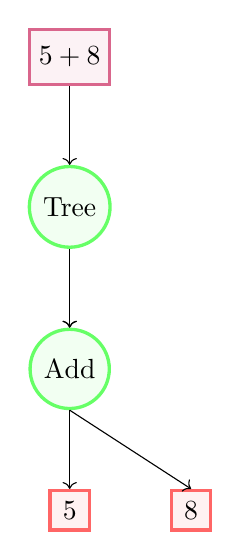
\begin{tikzpicture}[
equationnode/.style={rectangle, draw=purple!60, fill=purple!5, very thick, minimum size=7mm, align=center},
objectnode/.style={circle, draw=green!60, fill=green!5, very thick, minimum size=7mm, align=center},
variablenode/.style={rectangle, draw=red!60, fill=red!5, very thick, minimum size=5mm, align=center},
]
%Nodes
\node[equationnode]		(eqn)										{$5 + 8$};
\node[objectnode]		(treeobj)			[below=of eqn]			{\codeword{Tree}};
\node[objectnode]		(addobj)			[below=of treeobj]		{\codeword{Add}};
\node[variablenode]		(num1)				[below=of addobj]		{$5$};
\node[variablenode]		(num2)				[right=of num1]			{$8$};


%Lines
\draw[->] (eqn.south) -- (treeobj.north);
\draw[->] (treeobj.south) -- (addobj.north);
\draw[->] (treeobj.south) -- (addobj.north);
\draw[->] (addobj.south) -- (num1.north);
\draw[->] (addobj.south) -- (num2.north);
\end{tikzpicture}
\end{minipage}
\begin{minipage}{.4\textwidth}
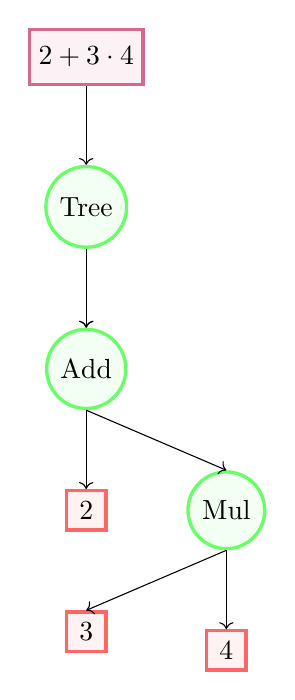
\begin{tikzpicture}[
equationnode/.style={rectangle, draw=purple!60, fill=purple!5, very thick, minimum size=7mm, align=center},
objectnode/.style={circle, draw=green!60, fill=green!5, very thick, minimum size=7mm, align=center},
variablenode/.style={rectangle, draw=red!60, fill=red!5, very thick, minimum size=5mm, align=center},
]
%Nodes
\node[equationnode]		(eqn)										{$2 + 3 \cdot 4$};
\node[objectnode]		(treeobj)			[below=of eqn]			{\codeword{Tree}};
\node[objectnode]		(addobj)			[below=of treeobj]		{\codeword{Add}};
\node[variablenode]		(num1)				[below=of addobj]		{$2$};
\node[objectnode]		(mulobj)			[right=of num1]			{\codeword{Mul}};
\node[variablenode]		(num2)				[below=of num1]			{$3$};
\node[variablenode]		(num3)				[below=of mulobj]		{$4$};


%Lines
\draw[->] (eqn.south) -- (treeobj.north);
\draw[->] (treeobj.south) -- (addobj.north);
\draw[->] (treeobj.south) -- (addobj.north);
\draw[->] (addobj.south) -- (num1.north);
\draw[->] (addobj.south) -- (mulobj.north);
\draw[->] (mulobj.south) -- (num2.north);
\draw[->] (mulobj.south) -- (num3.north);
\end{tikzpicture}
\end{minipage}
\begin{minipage}{.3\textwidth}
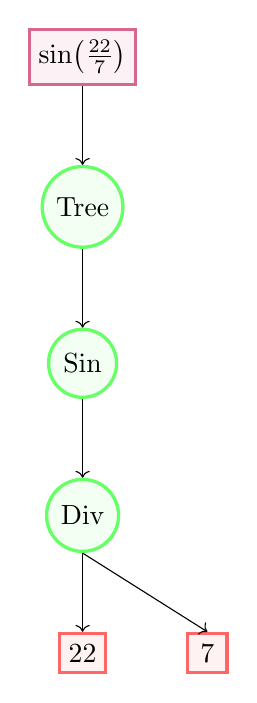
\begin{tikzpicture}[
equationnode/.style={rectangle, draw=purple!60, fill=purple!5, very thick, minimum size=7mm, align=center},
objectnode/.style={circle, draw=green!60, fill=green!5, very thick, minimum size=7mm, align=center},
variablenode/.style={rectangle, draw=red!60, fill=red!5, very thick, minimum size=5mm, align=center},
]
%Nodes
\node[equationnode]		(eqn)										{$\sin(\frac{22}{7})$};
\node[objectnode]		(treeobj)			[below=of eqn]			{\codeword{Tree}};
\node[objectnode]		(sinobj)			[below=of treeobj]		{\codeword{Sin}};
\node[objectnode]		(divobj)			[below=of sinobj]		{\codeword{Div}};
\node[variablenode]		(num1)				[below=of divobj]		{$22$};
\node[variablenode]		(num2)				[right=of num1]			{$7$};

%Lines
\draw[->] (eqn.south) -- (treeobj.north);
\draw[->] (treeobj.south) -- (sinobj.north);
\draw[->] (sinobj.south) -- (divobj.north);
\draw[->] (divobj.south) -- (num1.north);
\draw[->] (divobj.south) -- (num2.north);
\end{tikzpicture}
\end{minipage}

\subsection{Algorithms}

All high-level algorithms in \Symbo{} will operate recursively on the data they contain, and should not require external information to operate correctly.

For example, to evaluate the numeric result of an expression, the \codeword{eval} function will be called on the \codeword{Tree} object containing the equation. The \codeword{Tree} will then recursively call \codeword{eval} on the primary function/operation, which, in turn, calls \codeword{eval} on each of its branches. The numeric result of these function calls can then be propagated back up the tree, applying the relevant operations where necessary. This results in a final numeric result being returned from the \codeword{Tree} object.

\subsubsection{Example}

For example, if we evaluate the middle example from \ref{treeexample}:

\vspace{1cm}

\begin{minipage}{.33\textwidth}
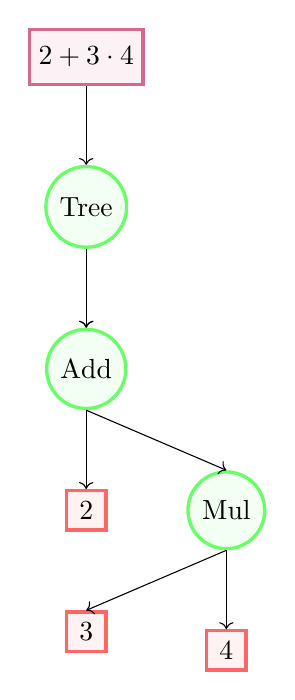
\begin{tikzpicture}[
equationnode/.style={rectangle, draw=purple!60, fill=purple!5, very thick, minimum size=7mm, align=center},
objectnode/.style={circle, draw=green!60, fill=green!5, very thick, minimum size=7mm, align=center},
variablenode/.style={rectangle, draw=red!60, fill=red!5, very thick, minimum size=5mm, align=center},
]
%Nodes
\node[equationnode]		(eqn)										{$2 + 3 \cdot 4$};
\node[objectnode]		(treeobj)			[below=of eqn]			{\codeword{Tree}};
\node[objectnode]		(addobj)			[below=of treeobj]		{\codeword{Add}};
\node[variablenode]		(num1)				[below=of addobj]		{$2$};
\node[objectnode]		(mulobj)			[right=of num1]			{\codeword{Mul}};
\node[variablenode]		(num2)				[below=of num1]			{$3$};
\node[variablenode]		(num3)				[below=of mulobj]		{$4$};


%Lines
\draw[->] (eqn.south) -- (treeobj.north);
\draw[->] (treeobj.south) -- (addobj.north);
\draw[->] (treeobj.south) -- (addobj.north);
\draw[->] (addobj.south) -- (num1.north);
\draw[->] (addobj.south) -- (mulobj.north);
\draw[->] (mulobj.south) -- (num2.north);
\draw[->] (mulobj.south) -- (num3.north);
\end{tikzpicture}
\end{minipage}
\begin{minipage}{.33\textwidth}
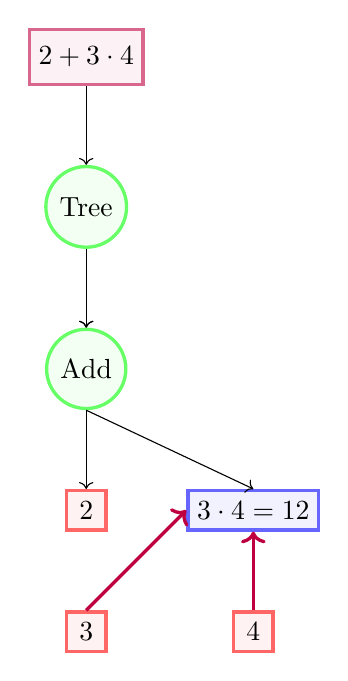
\begin{tikzpicture}[
equationnode/.style={rectangle, draw=purple!60, fill=purple!5, very thick, minimum size=7mm, align=center},
objectnode/.style={circle, draw=green!60, fill=green!5, very thick, minimum size=7mm, align=center},
variablenode/.style={rectangle, draw=red!60, fill=red!5, very thick, minimum size=5mm, align=center},
evalnode/.style={rectangle, draw=blue!60, fill=blue!5, very thick, minimum size=5mm, align=center},
]
%Nodes
\node[equationnode]		(eqn)										{$2 + 3 \cdot 4$};
\node[objectnode]		(treeobj)			[below=of eqn]			{\codeword{Tree}};
\node[objectnode]		(addobj)			[below=of treeobj]		{\codeword{Add}};
\node[variablenode]		(num1)				[below=of addobj]		{$2$};
\node[evalnode]			(mulobj)			[right=of num1]			{$3 \cdot 4 = 12$};
\node[variablenode]		(num2)				[below=of num1]			{$3$};
\node[variablenode]		(num3)				[below=of mulobj]		{$4$};


%Lines
\draw[->] (eqn.south) -- (treeobj.north);
\draw[->] (treeobj.south) -- (addobj.north);
\draw[->] (treeobj.south) -- (addobj.north);
\draw[->] (addobj.south) -- (num1.north);
\draw[->] (addobj.south) -- (mulobj.north);
\draw[purple, very thick, ->] (num2.north) -- (mulobj.west);
\draw[purple, very thick, ->] (num3.north) -- (mulobj.south);
\end{tikzpicture}
\end{minipage}
\begin{minipage}{.33\textwidth}
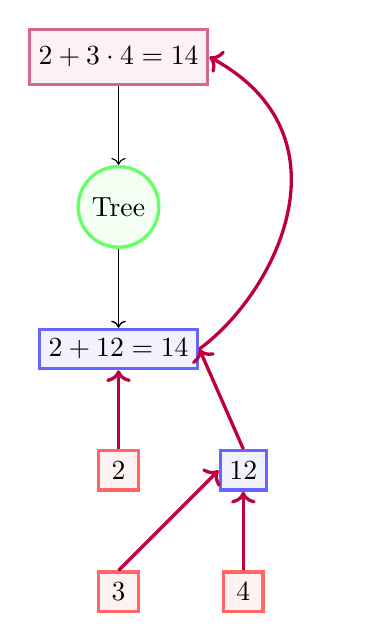
\begin{tikzpicture}[
equationnode/.style={rectangle, draw=purple!60, fill=purple!5, very thick, minimum size=7mm, align=center},
objectnode/.style={circle, draw=green!60, fill=green!5, very thick, minimum size=7mm, align=center},
variablenode/.style={rectangle, draw=red!60, fill=red!5, very thick, minimum size=5mm, align=center},
evalnode/.style={rectangle, draw=blue!60, fill=blue!5, very thick, minimum size=5mm, align=center},
]
%Nodes
\node[equationnode]		(eqn)										{$2 + 3 \cdot 4 = 14$};
\node[objectnode]		(treeobj)			[below=of eqn]			{\codeword{Tree}};
\node[evalnode]			(addobj)			[below=of treeobj]		{$2 + 12 = 14$};
\node[variablenode]		(num1)				[below=of addobj]		{$2$};
\node[evalnode]			(mulobj)			[right=of num1]			{$12$};
\node[variablenode]		(num2)				[below=of num1]			{$3$};
\node[variablenode]		(num3)				[below=of mulobj]		{$4$};


%Lines
\draw[->] (eqn.south) -- (treeobj.north);
\draw[->] (treeobj.south) -- (addobj.north);
\draw[->] (treeobj.south) -- (addobj.north);
\draw[purple, very thick, ->] (num1.north) -- (addobj.south);
\draw[purple, very thick, ->] (mulobj.north) -- (addobj.east);
\draw[purple, very thick, ->] (num2.north) -- (mulobj.west);
\draw[purple, very thick, ->] (num3.north) -- (mulobj.south);

%Curvy line :)
\draw[purple, very thick, ->] (addobj.east) .. controls(2, -3) and (3, -1) .. (eqn.east);
\end{tikzpicture}
\end{minipage}

\vspace{1cm}

Hopefully, the example above shows that it is possible to evaluate a tree recursively to calculate a numeric result. These steps can be extended to differentiation, simplification and potentially integration. 

\pagebreak

\subsection{External Libraries}

In order to reduce the chance of bugs appearing and to improve functionality, \Symbo{} makes use of a few external libraries.

\vspace{0.5cm}

\dirtree{%
	.1 \Symbo.
	.2 {LibRapid \cite{librapid} -- Provides advanced maths functionality}.
	.3 {MPFR \cite{MPFR} -- Support for multi-precision floating point types}.
	.3 {MPIR \cite{MPIR} -- Required by MPFR}.
	.2 {\{fmt\} \cite{fmt} -- For faster, easier string manipulation and printing}.
	.2 {scnlib \cite{scnlib} -- Provides fast string scanning and casting routines}.
}

\pagebreak

\section{Implementing the Data Types}

This section defines the abstract class interface for the different data types described in \ref{datatypes}. As mentioned there, each data type should hold only the data necessary for its operation, and efforts should be made to avoid global data accesses.

\subsection{The Component Type}

For the data structure identified in \ref{datatypes}, it is necessary to have a single base object which all other types will inherit from. This data type should have very minimal functionality, and all the functions it provides should ultimately be overwritten by the subclass.

Internally, the \codeword{Component} type contains virtual functions which throw an error when called, ensuring they cannot be called accidentally and cause unwanted results.

To start with, none of the classes will support any advanced features like simplification or calculus, but will support a simple, numeric evaluation function so we can check that the whole system is working correctly.

\begin{lstlisting}[language=C++]
virtual Scalar eval() const;
virtual std::string type() const;
virtual std::string name() const;
virtual std::string str(ui64 indent) const;
virtual std::string repr(ui64 indent,
                         ui64 typeWidth,
                         ui64 valWidth) const;
\end{lstlisting}

\subsubsection{Evaluation}

The \codeword{eval} function returns a scalar value, which is the result of evaluating the object. Note that all of these functions are \codeword{const}, and hence cannot change the data contained within the node. The evaluation function for each type will be covered later.

\subsection{Type Detection}

The \codeword{type} function returns the type of the object (i.e. \codeword{"NUMBER"}, \codeword{"VARIABLE"}, \codeword{"FUNCTION"}, etc.). This is used in the cases where more information needs to be known about a specific object, as the program cannot apply a general algorithm. It is also closely linked to the helper functions, and is used for debugging purposes.

\subsection{Naming}

Objects like functions and variables have names associated with them, and hence a procedure to extract the name of a given object is required. For objects which do not have a name associated with them, calling this function will raise an error, limiting unwanted behaviour.

\subsection{Helpers}

The \codeword{str} and \codeword{repr} functions are purely to debug the algorithms and ensure that everything is working correctly. They both return string representations of the object, but in slightly different formats, with different information.

\subsection{The Number Type}

The \codeword{Number} class is incredibly simple, and stores a single \codeword{Scalar} object (note that Scalar is typedef'ed, so it can represent any compile-time data type). The \codeword{eval} function simply returns the value stored in the class.

\begin{lstlisting}[language=C++]
class Number : public Component {
public:
	/* [ code omitted ] */
	
	Scalar eval() const override { return m_value; }
	
	/* [ code omitted ] */
private:
	Scalar m_value = 0;
};
\end{lstlisting}

\subsection{Variables}

Symbols such as $x$ and $y$ will be represented by the \codeword{Variable} class, which implements a few basic functions.

Firstly, the evaluation method of the class will always raise error, as, in this implementation, a variable must be replaced with a number in order to evaluate it. To support this replacement, the class supports a \codeword{Substitute} method, which uses a mapping of strings to objects, where the string is the variable name and the object is any \Symbo{} data type. Any references to the variables provided in the map will be replaced with their corresponding objects.

The variable class also implements a method to access the symbol's name, which is used in table lookups and when deciding how to differentiate or integrate the symbol.

\begin{lstlisting}[language=C++]
class Variable : public Component {
public:
	/* [ code omitted ] */
	
	std::string name() const override { return m_name; }
	
	/* [ code omitted ] */
private:
	std::string m_name = "NONAME";
};
\end{lstlisting}

\subsection{Functions}

The \codeword{Function} class is responsible for handing arithmetic operations such as addition and subtraction and single-argument functions like $\sin(x)$ and $\cos(y)$. The class can also be used to handle multi-argument functions like $\text{max}(x, y, z)$ if required.

\subsubsection{The Functor}

In order to maintain runtime-compatible evaluation and to reduce the complexity of the program, the functor member of the function objects will be an instance of the \CC standard library \codeword{function} type, which provides a simple way to wrap a lambda function.

As the function definition must be known at compile-time, the functor will take a list of \codeword{Scalar} objects and will return another \codeword{Scalar} object, which is the result of the calculation. This allows for arbitrarily many arguments to be passed to a function at runtime.

\subsubsection{Functor Arguments}

The \codeword{Function} class also needs to know what arguments it is operating on, and these must be set at runtime. For this reason, each instance of the class will store a list of \codeword{Component} pointers (remember, these could be numbers, variables or functions) -- one for each argument to the function.

One downside to this approach is that the number of arguments cannot be determined from the functor argument itself, so another member variable is required to store this information, with a function to access it.

\subsubsection{Function Evaluation}

In order to evaluate the result of the function, the arguments, which are still \codeword{Component} pointers, must first be evaluated and stored in a list. That list can then be fed directly into the functor object and the result can be returned.

\vspace{1cm}

\begin{lstlisting}[language=C++]
class Function : public Component {
public:
	/* [ code omitted ] */

	Scalar eval() const override {
		std::vector<Scalar> operands;
		for (const auto &val : m_values)
			operands.push_back(val->eval());
		return m_functor(operands);
	}

	uint64_t numOperands() const { return m_numOperands; }

	std::string name() const override { return m_name; }

	/* [ code omitted ] */

private:
	std::string m_name	 = "NULLOP";
	std::function<Scalar(const std::vector<Scalar> &)> m_functor;
	uint64_t m_numOperands = 0;

	std::vector<std::shared_ptr<Component>> m_values = {};
};
\end{lstlisting}

\subsection{The Tree Type}

The \codeword{Tree} class is mainly intended to store a single function object which can then be evaluated. It also provides a few helper functions to format equations, though these are purely visual and have no impact on the program itself.

In the code listing, you may notice that the \codeword{m_tree} member is a list of pointers; this is done for future-proofing to allow variable values to be stored on a per-equation basis, for example. However, this currently serves no purpose and can easily be changed to store a single object.

\vspace{0.25cm}

\begin{lstlisting}[language=C++]
class Tree : public Component {
public:
	/* [ code omitted ] */

	Scalar eval() const override { return m_tree[0]->eval(); }
	
	/* [ code omitted ] */
private:
	std::vector<std::shared_ptr<Component>> m_tree;
};
\end{lstlisting}

\pagebreak

\section{Processing the Equation Input}

Before it is possible to generate the tree from the input equation (in this case, a \codeword{std::string}), the text must first be processed into a form that can be understood more easily by the computer.

\subsection{Tokenizing}

The first step in transforming the user's input into something the computer can process is called ``tokenizing''\footnote{Tokenizing and lexing are technically the same process, however, in \Symbo{} the process is split into two parts, and ``tokenizing'' fits the first part more closely than ``lexing''.}. It is the process of splitting the input string into a list of ``tokens'', which, in this case, are individual characters \footnote{``Character'' in reference to ASCII characters -- i.e., not limited to letters of the alphabet.} the program is allowed to use.

The process is very simple, and involves iterating over each character in the input text, checking whether it's a valid character to be in an equation (e.g. emojis are invalid) and, if it is, storing it in a list. This process also removes spaces from the input, as they are not important to the equation itself.

Another data type is required to store the result of this process, which contains information about the type of the value stored, along with the actual character.

\begin{lstlisting}[language=C++, caption={The token object definition}]
struct Token {
	uint64_t type;
	char val;
};
\end{lstlisting}

\subsubsection{Example} \label{tokenexample}

For example, the input $12 + 3$ will produce the list of tokens shown below. Note, however, that \codeword{TYPE_DIGIT}, \codeword{TYPE_ADD} and \codeword{TYPE_OPERATION} are all numeric values.

\begin{lstlisting}[language=C++]
// ===== [ 0 ] =====
{
	uint64_t type = TYPE_DIGIT;
	char val      = '1';
}
// ===== [ 1 ] =====
{
	uint64_t type = TYPE_DIGIT;
	char val      = '2';
}
// ===== [ 2 ] =====
{
	uint64_t type = TYPE_ADD | TYPE_OPERATION;
	char val      = '+';
}
// ===== [ 3 ] =====
{
	uint64_t type = TYPE_DIGIT;
	char val      = '3';
}
\end{lstlisting}

\subsection{Lexing}

The individual characters returned from the tokenizing step are entirely useless unless we can make sense of what they mean in a larger context. This is the task of the ``lexer'', which takes the characters identified in the previous step and produces a list of objects which the computer can easily make sense of.

The lexer algorithm itself is quite simple, and joins together strings of digits to form numbers, strings of characters to form text and identifies arithmetic operations and brackets.

Another data type is also required for the output of the lexing process. It is almost exactly the same as the token object, except that it stores a string instead of a single character.

Taking the example given in \ref{tokenexample}, the algorithm will output the following.

\begin{lstlisting}[language=C++]
// ===== [ 0 ] =====
{
	uint64_t type   = TYPE_NUMBER | TYPE_VARIABLE;
	std::string val = "12";
}
// ===== [ 1 ] =====
{
	uint64_t type   = TYPE_ADD | TYPE_OPERATION;
	std::string val = "+";
}
// ===== [ 2 ] =====
{
	uint64_t type   = TYPE_NUMBER | TYPE_VARIABLE;
	std::string val = "3";
}
\end{lstlisting}

\subsection{Processing the Lexed Results}

This section of the program isn't necessarily required, but it will serve a very important purpose later down the line, as well as allowing for a few more mathematical inputs.

When writing an equation by hand, it is not uncommon to write something like $5(3x-2)$ or $2\sin(x)$. In these cases, we understand that the term preceded by a coefficient should be multiplied by that coefficient, however the computer will not currently understand this.

To simplify things, a \codeword{Lexed{TYPE_MUL, "*"}} can be inserted between the coefficient and the rest of the term, leaving it completely unchanged from a mathematical point of view, but making it much easier for the later stages to use.

We also need to check for equations like $x(5+y)$, however this is more complicated as it is not always possible to check for text followed by an open bracket. To show why, take the expression $\sin(x)$ -- using the naive method from above will lead to $\text{sin} \cdot x$, which is obviously not a valid equation.

To mitigate this issue, \Symbo{} stores a list of all defined functions, and checks whether the value preceding the bracket is registered as one. If no corresponding function is found, it can be assumed that the value is referring to a variable; the value of which will be specified when the equation is evaluated. In this case, a multiplication can safely be inserted between the coefficient and the rest of the term. 

If the value is identified as a registered function, further modification is required.

\subsection{Conversion to Postfix Notation}

Currently, the equations are in ``infix'' form, which refers to how we normally write equations, where the operator sits between the two operands.

One downside of representing equations with infix notation is that the operator precedence plays a large role in the final result. While it is possible to process equations in this form directly, converting them to ``postfix'' notation dramatically simplifies the tree generation algorithm.

\subsubsection{Postfix Notation}

Postfix notation (sometimes called ``Reverse Polish Notation'') places the operator after the operands, and relies on a stack-based approach to calculate the final result. Postfix notation also removes the requirement for brackets, as the order of precedence is implied by the order of the operations in the equation.

Below are three different examples of postfix notation:

\begin{equation}
\begin{split}
\text{Infix} \ & \ \ \ \ \text{Postfix} \\
5+10&=5 \ 10 \ + \\
\left( 1+2 \right) \cdot 3&=1 \ 2 \ + \ 3 \ \cdot \\
2 + 3 \cdot 4 ^ x&=2 \ 3 \ 4 \ x \ \textit{pow} \ \cdot \ +
\end{split}
\end{equation}

To evaluate the result, start on the first number and push it to the stack -- repeat this until an operator is found. The operator acts on $n$ values, so pop off the top $n$ items from the stack, apply the operation to those $n$ values and push the result back onto the stack. Repeat this until the stack is empty.

\subsubsection{Infix to Postfix}

To convert from infix to postfix notation, we can use Dijkstra's ``Shunting Yard Algorithm''\cite{shuntingyard}, which acts as follows:

\begin{algorithm}
\caption{Dijkstra's Shunting Yard Algorithm}\label{shuntingalgorithm}
\begin{algorithmic}[1]
\Function{to\_postfix}{$\textit{input}$}\Comment{Convert from infix to postfix}
	\State $\textit{postfix} \gets \{\}$
	\State $\textit{stack} \gets \{\}$
	\For{$\textit{lex} \ \textbf{in} \ \textit{input}$}
		\If{$\textit{lex} \rightarrow \textit{type} \ \textbf{is} \ \textit{variable}$} \Comment{Number or string}
			\State $\textit{postfix} \ \textbf{push back} \ \textit{lex}$
		\ElsIf{$\textit{lex} \rightarrow \textit{type} \ \textbf{is} \ \textit{(operator, function)}$}
			\While{$\textit{stack} \ \textbf{not empty} \ \textbf{and} \ \textit{stack} \rightarrow \textit{back} \rightarrow \textit{precedence} \ \ge \ \textit{lex} \rightarrow \textit{precedence}$}
				\State $\textit{postfix} \ \textbf{push back} \ \textit{stack} \rightarrow \textit{back}$
				\State $\textbf{pop} \ \textit{stack}$
			\EndWhile
			\State $\textit{stack} \ \textbf{push back} \ \textit{lex}$
		\ElsIf{$\textit{lex} \rightarrow \textit{type} \ \textbf{is} \ \textit{leftparen}$}
			\State $\textit{stack} \ \textbf{push back} \ \textit{lex}$ \Comment{Store the bracket for later}
		\ElsIf{$\textit{lex} \rightarrow \textit{type} \ \textbf{is} \ \textit{rightparen}$}
			\While{$\textit{stack} \rightarrow \textit{back} \ \textbf{is not} \ \textit{leftparen}$} 
				\State $\textit{postfix} \ \textbf{push back} \ \textit{stack} \rightarrow \textit{back}$
			\EndWhile
			\State $\textbf{pop} \ \textit{stack}$ \Comment{Remove the left bracket}
		\EndIf
	\EndFor\
	\While{$\textit{stack} \ \textbf{not empty}$} \Comment{Pop remaining operators}
		\State $\textit{postfix} \ \textbf{push back} \ \textit{stack} \rightarrow \textit{back}$
		\State $\textbf{pop} \ \textit{stack}$
	\EndWhile
\EndFunction
\end{algorithmic}
\end{algorithm}

\pagebreak

\subsection{Parsing}

The final stage is to parse the resulting objects. This process involves identifying whether the object is a number, a variable or a function, and mapping it to the correct type for the system to understand it.

\subsubsection{Numbers}

If the lexed type is a number, \Symbo{} simply outputs a \linebreak \codeword{std::make_shared<Number>(lex.val)}.

\subsubsection{Strings}

A string could represent either a variable or a function. \Symbo{} operates on the premise that functions must be declared before the equation is constructed, but variables can be specified afterwards, meaning the program must check if the string exists as a function and otherwise assumes it is a variable.

\begin{lstlisting}[language=C++, caption={Convert from text to either a function or variable}]
auto func = findFunction(lex.val);
if (func != functions.end()) {
	res.emplace_back(*func);
} else {
	res.emplace_back(std::make_shared<Variable>(lex.val));
}
\end{lstlisting}

\subsubsection{Operators}

Arithmetic operators are also functions, so a simple lookup is all that is needed. To reduce bugs, the code still checks whether the functions were successfully found, as it's possible the functions haven't been registered at this point in the program. \Symbo{} will throw an error if this is the case.

\begin{lstlisting}[language=C++, caption={Identify arithmetic operators and convert them to function objects}]
auto func = findFunction("_"); // Default to a nullary function
if (lex.type & TYPE_ADD) func = findFunction("ADD");
if (lex.type & TYPE_SUB) func = findFunction("SUB");
if (lex.type & TYPE_MUL) func = findFunction("MUL");
if (lex.type & TYPE_DIV) func = findFunction("DIV");
if (lex.type & TYPE_CARET) func = findFunction("POW");
LR_ASSERT(func != functions.end(), "Operator not found");
res.emplace_back(*func);
\end{lstlisting}

\pagebreak

\section{Equation Tree Generation}

With the equations in postfix notation, it would be quite trivial to evaluate a numeric result with no further manipulation, however, to work with variables, implement calculus and more advanced manipulations, it will be necessary to transform the equation into a tree-like structure.

To do this, we can evaluate the postfix equation and apply the typing system implemented earlier to store the final equation, instead of evaluating it numerically.

\begin{algorithm}
\caption{Postfix to Tree}\label{treegenalg}
\begin{algorithmic}[1]
\Function{gen\_tree}{$\textit{input}$}\Comment{Generate a tree from postfix notation}
	\State $\textit{tree} \gets \textit{empty tree}$
	\State $\textit{stack} \gets \textit{empty stack}$
	
	\For{$\textit{lex} \ \textbf{in} \ \textit{input}$}
		\If{$\textit{lex} \rightarrow \textit{type} \ \textbf{is} \ \textit{(number, variable)}$}
			\State $\textit{stack} \ \textbf{push back} \ \textit{lex}$
		\ElsIf{$\textit{lex} \rightarrow \textit{type} \ \textbf{is} \ \textit{function}$}
			\State $\textit{args} \gets \textit{\{\}}$
			\For{$i \ \textbf{in} \ 0..(\textit{lex} \rightarrow \textit{numOperands})$}
				\State $\textit{args} \ \textbf{push back} \ \textit{stack} \rightarrow \textit{back}$
				\State $\textbf{pop} \ \textit{stack}$
			\EndFor			
			
			\State $\textit{node} \gets \textbf{copy} \ \textit{lex}$ \Comment{lex is a function}
			
			\For{$arg \ \textbf{in} \ \textbf{reverse} \ \textit{args}$}
				\State $\textit{node} \ \textbf{add value} \ \textit{arg}$
			\EndFor				
			
			\State $\textit{stack} \ \textbf{push back} \ \textit{node}$ \Comment{Push node back onto stack}
		\EndIf
	\EndFor
	
	\State $\textit{tree} \ \textbf{set node} \ \textit{stack} \rightarrow \textit{back}$
\EndFunction
\end{algorithmic}
\end{algorithm}

\pagebreak

As an example, we can test the algorithm on the trees from \ref{treeexample}. Each of the three examples below shows the input to the program, the generated tree and the numeric result after calling \codeword{eval} on the main tree object.

\subsection{Example 1}
\begin{lstlisting}[language=C++]
Input: "5 + 8"
[ TREE ]
    [ FUNCTION ] [ ADD ]
        [ NUMBER ] [ 5.0000000000 ]
        [ NUMBER ] [ 8.0000000000 ]
        
Result: 13
\end{lstlisting}

\subsection{Example 2}
\begin{lstlisting}[language=C++]
Input: "2 + 3 * 4"
[ TREE ]
    [ FUNCTION ] [ ADD ]
        [  NUMBER  ] [ 2.0000000000 ]
        [ FUNCTION ] [     MUL      ]
            [ NUMBER ] [ 3.0000000000 ]
            [ NUMBER ] [ 4.0000000000 ]
            
Result: 14
\end{lstlisting}

\subsection{Example 2}
\begin{lstlisting}[language=C++]
Input: "sin(22 / 7)"
[ TREE ]
    [ FUNCTION ] [ sin ]
        [ FUNCTION ] [ DIV ]
            [ NUMBER ] [ 22.0000000000 ]
            [ NUMBER ] [ 7.0000000000  ]
            
Result: -0.00126448893037729 
\end{lstlisting}

\pagebreak

\section{Variables}

Currently, \Symbo{} can store variables in the tree, but cannot process them in any way. The first step to having full support for variables to allow an equation to be evaluated with substitutions for variables.

\subsection{Numeric Variable Evaluation}

Providing values for variables involves passing in a set of name-value pairs, such as \codeword{("x", 123)}, which can tell \Symbo{} what to substitute in place of variables. To make this process easier, \Symbo{} needs a function to convert an input value into one of a number, a variable or a tree, depending on what is passed to it.

\begin{algorithm}
\caption{Intelligent automatic parsing system}\label{treegenalg}
\begin{algorithmic}[1]
\Function{auto\_parse}{$\textit{input}$}
	\If{$textit{input} \ \textbf{is} \ \textit{(number, variable)}$}
		\State $\textbf{return} \ \textit{input}$ \Comment{Leave the input as a number of variable}
	\Else
		\State $\textbf{return} \ \textbf{gentree} \ \textit{input}$ \Comment{Generate a new tree object}
	\EndIf
\EndFunction
\end{algorithmic}
\end{algorithm}

By developing a function similar to \codeword{eval} which, instead of generating numeric results, produces a new \codeword{Tree} object where all instances of a given variable are replaced with their corresponding expansions.

Additionally, this implementation allows for another equation to be passed as a variable. This could be used to substitute a rearranged equation into another, for example.

\subsubsection{Example}
\begin{lstlisting}[language=C++]
Input: "a * b" with {"a": "5", "b": "2 + 4"}

Original Tree:
[ TREE ]
    [ FUNCTION ] [ MUL ]
        [ VARIABLE ] [ a ]
        [ VARIABLE ] [ b ]
        
Substituted Tree:
[ TREE ]
    [ FUNCTION ] [ MUL ]
        [ NUMBER ] [ 5 ]
        [ FUNCTION ] [ ADD ]
            [ NUMBER ] [ 2 ]
            [ NUMBER ] [ 4 ]
        
Result: 30
\end{lstlisting}

\subsection{Pretty Printing an Equation}

While the tree representation of an equation is useful in some ways, it is not how we are used to viewing an equation. For this reason, a \codeword{prettyPrint} function is needed, which will format a \codeword{Tree} object more nicely.

The internal workings of the function are not important here, but it uses some logic to ensure brackets are placed where they are needed (and sometimes where they are \textit{not} needed, though are still valid).

\subsubsection{Example}

\begin{lstlisting}[language=C++]
Input: "(2 * 3 + 4) / sin(x)"
Pretty Printed: ((2 * 3) + 4) / (sin(123))
(note the extra brackets)
\end{lstlisting}

\pagebreak

\section{Differentiation}

Differentiation is a very useful tool in mathematics, and, fortunately, can be implemented into \Symbo{} relatively easily.

Luckily, almost any equation can be differentiated using a small subset of rules, as these rules can be applied to smaller and smaller parts of the equation until the final result is generated.

\Symbo{} will differentiate the tree object recursively, similar to how the tree is evaluated.

\subsection{Differentiation Rules}

Below is the list of rules which can be used to differentiate any equation including addition, subtraction, multiplication and division. Other rules of differentiation for exponents and roots, trigonometry, logarithms, etc. will be implemented later, as no single identity exists for $a^b$ for any $a$ and $b$, for example.

\iftrue
\begin{equation}
\dv{x}a = 0, \ \text{for} \ a \in \mathbb{R}
\end{equation}

\begin{equation}
\dv{x}(f(x) \pm h(x)) = \dv{f}{x} \pm \dv{h}{x}
\end{equation}

\begin{equation}
\dv{x}{y}f(x)h(x) = v \dv{h}{x} + u \dv{f}{x}
\end{equation}

\begin{equation}
\dv{x}{y}\frac{f(x)}{h(x)} = \frac{h \dv{f}{x} - f \dv{h}{x}}{h^2}
\end{equation}

\begin{equation}
\dv{x}{y}\log{x} = \frac{1}{x}
\end{equation}
\fi

\iffalse
\begin{align*}
\dv{x}(f(x) \pm h(x)) &= \dv{f}{x} \pm \dv{h}{x}
\\
\\
\dv{x}{y}f(x)h(x) &= v \dv{h}{x} - u \dv{f}{x}
\\
\\
\dv{x}{y}\frac{f(x)}{h(x)} &= \frac{v \dv{u}{x} - u \dv{v}{x}}{v^2}
\end{align*}
\fi

\subsubsection{Implementing the Rules}

The rules, just like the number, variable and function types, will be implemented as classes which inherit from a single base type. This will allow them to be stored as pointers in an array, which can be iterated over to check each available rule.

Each rule will have two main methods: \codeword{applicable} and \codeword{derivative}; the first of which will detect whether a given rule can be applied to an object, and the second of which applies the actual operation.

The return value from the \codeword{derivative} function will be a \codeword{Tree} object containing the relevant operations and operands, though not necessarily in it's simplest form.

\subsubsection{Problems With This Implementation}

As mentioned earlier, using generic rules in this form will not result in neat derivatives. For example, using the above rules, differentiating $5x + 2$ will output $((0 \cdot x) + (5 \cdot 1)) + 0$. This, of course, simplifies to $5$, however \Symbo{} currently has no way of applying such a simplification.

Upon observation of more generated derivatives, it's clear that the most common area for improvement is removing multiplications by zero or one, additions or subtractions of zero and other simple arithmetic operations. This leads us to develop a simple set of rules for the initial simplification of an equation

\pagebreak

\section{Simplification of Equations}

Implementing equation simplification could be done in many different ways, though the most effective, given the current data layout, is almost identical to the differentiation implementation.

A single class will define the base \codeword{SimplificationRule} type, and all implementations will inherit from this type, allowing a list of generic rule types to be stored in a list and utilised.

Similar to the differentiation set up, each simplification rule will implement two methods: \codeword{isApplicable} and \codeword{simplify}.

In order to clean up the most basic equations, only a small set of rules are needed:

\begin{itemize}
	\item Any branch involving only numbers gets evaluated
	\item $x \pm 0 = x$
	\item $0 + x = x$
	\item $0 - x = -x$
	\item $x \cdot 0 = 0$
	\item $x \cdot 1 = x$
	\item $\frac{0}{x} = 0 \ \text{where} \ x \neq 0$
	\item $\frac{x}{1} = x$
\end{itemize}

\vspace{0.25cm}

By applying these rules recursively from the bottom of the tree upwards, simple issues in equations (mainly the results of derivatives) can be eliminated. The implementation of this is identical to that of the differentiation algorithm.

\subsection{Example}

\begin{lstlisting}[language=C++]
Input: "1/x"
Derivative (original): "((0 * x) - (1 * 1)) / (x ^ 2)"
Derivative (simplified): "-1 / (x ^ 2)"
\end{lstlisting}

\pagebreak

\section{Further Issues and Potential Remedies}

While this implementation of a symbolic mathematics library is relatively basic in terms of the maths it can actually perform, the fundamental concepts can easily be expanded on to produce a much more complete system.

While many of these features are beyond the scope of this project, the methodology for providing solutions to some issues are explained below.

\subsection{More Advanced Functions}

The current \Symbo{} function object operates in \CC, not \Symbo's data types. This means that all functions must be implemented as \CC code and hence cannot be created and modified at runtime.

For example, adding a custom function $f(x) = 5x+3$ would require the instantiation of a new \codeword{Function} object, and would prevent the creation of a new function with the same name.

To get around this issue, one could create a new \codeword{UserFunction} class which allows for custom definitions of functions, though this is a convoluted approach and is likely to cause more problems down the line.

Ideally, the system would natively support most common mathematical concepts, including basic arithmetic, exponents and logarithms, trigonometry, etc., and all other functions would be defined in terms of that basic set of operations. This would include things such as $\csc(x)$ and $\sec(x)$, for example, which would be defined as $\left(\sin(x)\right)^{-1}$ and $\left(\cos(x)\right)^{-1}$ respectively.

\subsection{Differentiation}

Based purely on the implementation outlined in this paper, a program would be limited to differentiating equations including only arithmetic operations and real exponents. This is not acceptable for a program being used in advanced calculations.

Implementing more advanced derivatives would simply mean applying more rules to the program. A good start to this would be implementing derivatives for logarithms, exponentials and trigonometric functions.

More generally, an ideal solution would be to state a single derivative $f'(x)=g(x)$ for a given function $f(x)$, all defined given the advanced function implementation described above. From here, generic function rules such as $\dv{h}{x} h(a) = \dv{a}{x} \cdot h'(a)$ to extrapolate the rule to a broader range of equations.

Hopefully it is clear that, to differentiate advanced equations, a program merely needs to define a suitably large number of differentiation rules.

\subsection{Integration}

Integrating equations is much more difficult than differentiating them, and involves some complex tricks and assumptions \cite{mathematicainternals} which are too complicated to implement in this paper.

Often, integrating symbolically requires testing a wide range of different substitutions and applying a set of known integration rules to the manipulated equation. It is unlikely that such an implementation would act recursively, however, so the existing infrastructure of the system would not be useful.

\subsection{Simplification}

Simplification of equations, similar to differentiation, is limited almost entirely by the set of rules available to the program. Given enough rules, the algorithm would be capable of simplifying almost anything.

If this were combined with a rearrangement algorithm to suggest different permutations of equations, this could become even more powerful.

\subsubsection{Example}

\begin{lstlisting}[language=C++]
Input: "5x^2 + 3x + 2"
Derivative: "(5 * (2 * x)) + 3"
\end{lstlisting}

In the above case, the $5\cdot(2\cdot x)$ should, of course, be simplified down to $10x$. This could be achieved by implementing a rule in the \codeword{SimplifyMul} class to look for scalar scale factors, for example.

\pagebreak

\section{Conclusion}

This paper explores a potential implementation of a symbolic mathematics library in \CC, a statically-typed, compiled language. The program, \Symbo, avoids the issues of static typing by employing a polymorphic approach using the standard library's shared pointer type.

The implementation of this library shows that it is possible to process equations involving symbols and functions without directly evaluating a numeric result at each step, as well as identifying methods for substituting values, assigning values to variables, differentiating and simplifying equations.

While there are many areas in which this implementation is complete, it could easily be expanded to support a wider range of equations and functions, as well as potentially solving some types of equations by rearranging and manipulating equations.

\subsection{Benchmarks}

In addition to this implementation's functionality, it is also relatively quick for a pointer-based approach, taking a matter of microseconds for most stages of the equation processing.

\vspace{0.25cm}

\begin{center}
\begin{tabular}{||c c c c c||} 
 \hline
 Input & GenTree & Diff & Simplify Diff & Eval\\ [0.5ex] 
 \hline\hline
 $5x + 2$ & $\SI{3.829}{\micro\second}$ & $\SI{1.804}{\micro\second}$ & $\SI{1.906}{\micro\second}$ & $\SI{1.007}{\micro\second}$ \\ 
 \hline
 $(5x + 2) \cdot (3x - 1)$ & $\SI{14.282}{\micro\second}$ & $\SI{5.759}{\micro\second}$ & $\SI{7.255}{\micro\second}$ & $\SI{2.321}{\micro\second}$ \\ 
 \hline
 $\left( \frac{(x^2 - x - 1)}{(x^2 + x + 1)} \right)^5$ & $\SI{15.225}{\micro\second}$ & $\SI{13.436}{\micro\second}$ & $\SI{23.247}{\micro\second}$ & $\SI{4.810}{\micro\second}$ \\   [1ex] 
 \hline
\end{tabular}
\end{center}

\pagebreak

\begin{thebibliography}{X}
\bibitem{symbolicdefinition} TheFreeDictionary.com. (n.d.). symbolic mathematics. [online] Available at: \href{https://encyclopedia2.thefreedictionary.com/symbolic+mathematics}{https://encyclopedia2.thefreedictionary.com/symbolic+mathematics} [Accessed 9 Aug. 2022].

\bibitem{mathematica} Wolfram.com. (2019). Wolfram Mathematica. [online] Available at: \href{https://www.wolfram.com/mathematica/}{https://www.wolfram.com/mathematica/}.

\bibitem{riemannsum} Weisstein, E.W. (n.d.). Riemann Sum. [online] mathworld.wolfram.com. Available at: \href{https://mathworld.wolfram.com/RiemannSum.html}{https://mathworld.wolfram.com/RiemannSum.html}.

\bibitem{sympy} www.sympy.org. (n.d.). SymPy. [online] Available at: \href{https://www.sympy.org/en/index.html}{https://www.sympy.org/en/index.html}.

\bibitem{computeraidformathematics} Clapp, L.C. and Kain, R.Y. (1963). A computer aid for symbolic mathematics. Proceedings of the November 12-14, 1963, fall joint computer conference on XX - AFIPS ’63 (Fall). doi:10.1145/1463822.1463877.

\bibitem{githubmathlibs} GitHub.com (n.d.). Build software better, together. [online] Available at: \href{https://github.com/topics/symbolic-math?l=c\%2B\%2B}{https://github.com/topics/symbolic-math?l=c\%2B\%2B} [Accessed 9 Aug. 2022].

\bibitem{mathiucpp} Fu, B. (2022). mathiu.cpp. [online] GitHub. Available at: \href{https://github.com/BowenFu/mathiu.cpp}{https://github.com/BowenFu/mathiu.cpp} [Accessed 10 Aug. 2022].

\bibitem{symengine} GitHub. (2022). SymEngine. [online] Available at: \href{https://github.com/symengine/symengine}{https://github.com/symengine/symengine} [Accessed 4 Oct. 2022].

\bibitem{mathematicainternals} reference.wolfram.com. (n.d.). The Internals of the Wolfram System—Wolfram Language Documentation. [online] Available at: \href{https://reference.wolfram.com/language/tutorial/TheInternalsOfTheWolframSystem.html}{https://reference.wolfram.com/language/tutorial/ TheInternalsOfTheWolframSystem.html} [Accessed 10 Aug. 2022].

‌\bibitem{librapid} Davis, T. (2022). LibRapid: Optimised Mathematics for \CC (Version 0.5.2) [Computer software]. \href{https://github.com/LibRapid/librapid}{https://github.com/LibRapid/librapid}

‌\bibitem{MPFR} Fousse, L., Hanrot, G., Lefèvre, V., Pélissier, P. and Zimmermann, P. (2007). MPFR. ACM Transactions on Mathematical Software, 33(2), p.13. doi:10.1145/1236463.1236468.

‌\bibitem{MPIR} B. Gladman, W. Hart, J. Moxham, et al. MPIR: Multiple Precision Integers and Rationals, 2015. version 2.7.0, A fork of the GNU MP package (T. Granlund et al.) \href{http://mpir.org}{http://mpir.org}.

\bibitem{fmt} fmtlib (2019). fmtlib/fmt. [online] GitHub. Available at: \href{https://github.com/fmtlib/fmt}{https://github.com/fmtlib/fmt}.

\bibitem{scnlib} Kosunen, E. (2022). scnlib. [online] GitHub. Available at: \href{https://github.com/eliaskosunen/scnlib}{https://github.com/eliaskosunen/scnlib} [Accessed 11 Aug. 2022].‌

\bibitem{shuntingyard} Steingartner, William \& Yar-Muhamedov, Iskender. (2018). Learning software for handling the mathematical expressions. Journal of Applied Mathematics and Computational Mechanics. 17. 77-91. 10.17512/jamcm.2018.2.07. 

\end{thebibliography}
\end{document}
